\chapter{Design of the control system}\label{ch:ch4}

In the previous chapters, we outlined deep reinforcement learning fundamentals with its most critical underlying concepts, and then we discussed the choice made about the technologies to use as baselines for our experiments.
The decision fell on Anki Cozmo because of the high-quality SDK provided to developers and the versatility and flexibility provided by PyTorch, especially in a research context.

The following step in the path of this thesis consists of merging reinforcement learning theory with tools and frameworks presented previously to create the system in question.
Indeed, this chapter aims to describe the design of the control system for reinforcement learning experiments with Anki Cozmo.
The work presented in this part represents one of the contributions of our thesis and the necessary step towards reinforcement learning experiments.

The outline of the whole ecosystem with the description of interfaces, frameworks and technologies used occupies the first section of the chapter.
This part also comprehends a discussion about DDPG~\cite{lillicrap2015continuous} and SAC~\cite{haarnoja2018soft, haarnoja2018alg} implementation with references to the choice made in terms of hyper-parameters and problems faced.

The second part of the chapter aims to describe the implementation of Anki Cozmo OpenAI Gym environment from the problem formalisation as MDP to the implementation of human-robot interaction.

In the final section of this chapter, the design and setup of the real track will be discussed together with a discussion about the problems faced and the choice made to overcome them.

\section{Outline of the system}\label{sec:outline-of-the-system}

The development of the control system for Anki Cozmo was the main contribution of the thesis, together with the implementation of DDPG and SAC algorithm.
The main aim of this work was to create an OpenAI Gym environment capable of interacting with a robot in the real world, not just through the usage of a simulator.
OpenAI Gym usually provides plain and straightforward interfaces to interact with simulated environments: we decided to exploit these functions to allow the application of reinforcement learning algorithm directly in the real-world decision of the robot.

The fundamental source of inspiration to develop this control system was~\cite{kendall2018learning,kendall2019learning}.
This publication represents, as its authors reported, the first reinforcement learning self-driving experiment where a car learned to drive through the application of a reinforcement learning algorithm, by trial and error.
They first trained the model exploiting Deep Deterministic Policy Gradient (DDPG) in a simulator for many epochs and, after this learning process, they managed to transfer the knowledge acquired in the simulator in real-world experiments.

We decided to export and implement these ideas in our project, adapting them to the specificities and particularities of the Cozmo setup.
The resulting system can be summed up by~\vref{fig:system} which provide a schematic overview of every technology employed and the interaction among them.
This section aims to describe as clearly as possible all the components of the control system we designed.

\tikzset{every picture/.style={line width=0.75pt}} %set default line width to 0.75pt        

\begin{figure}
    \tikzset{every picture/.style={line width=0.75pt}} %set default line width to 0.75pt
    \centering
    \scalebox{0.75}{


        \tikzset{every picture/.style={line width=0.75pt}} %set default line width to 0.75pt

    \begin{tikzpicture}[x=0.75pt,y=0.75pt,yscale=-1,xscale=1]
        %uncomment if require: \path (0,438); %set diagram left start at 0, and has height of 438

        %Image [id:dp06991158821872456]
        \draw (239.75,55) node  {
\includegraphics[width=115.13pt,height=52.5pt]{img/python.png}};
        %Image [id:dp3729269645681633]
        \draw (240.25,198.5) node  {
\includegraphics[width=46.88pt,height=50.25pt]{img/gym.png}};
        %Image [id:dp09149607927009118]
        \draw (94.75,200.91) node  {
\includegraphics[width=124.13pt,height=25.37pt]{img/pytorch.png}};
        %Image [id:dp30806594376010465]
        \draw (351.92,200) node  {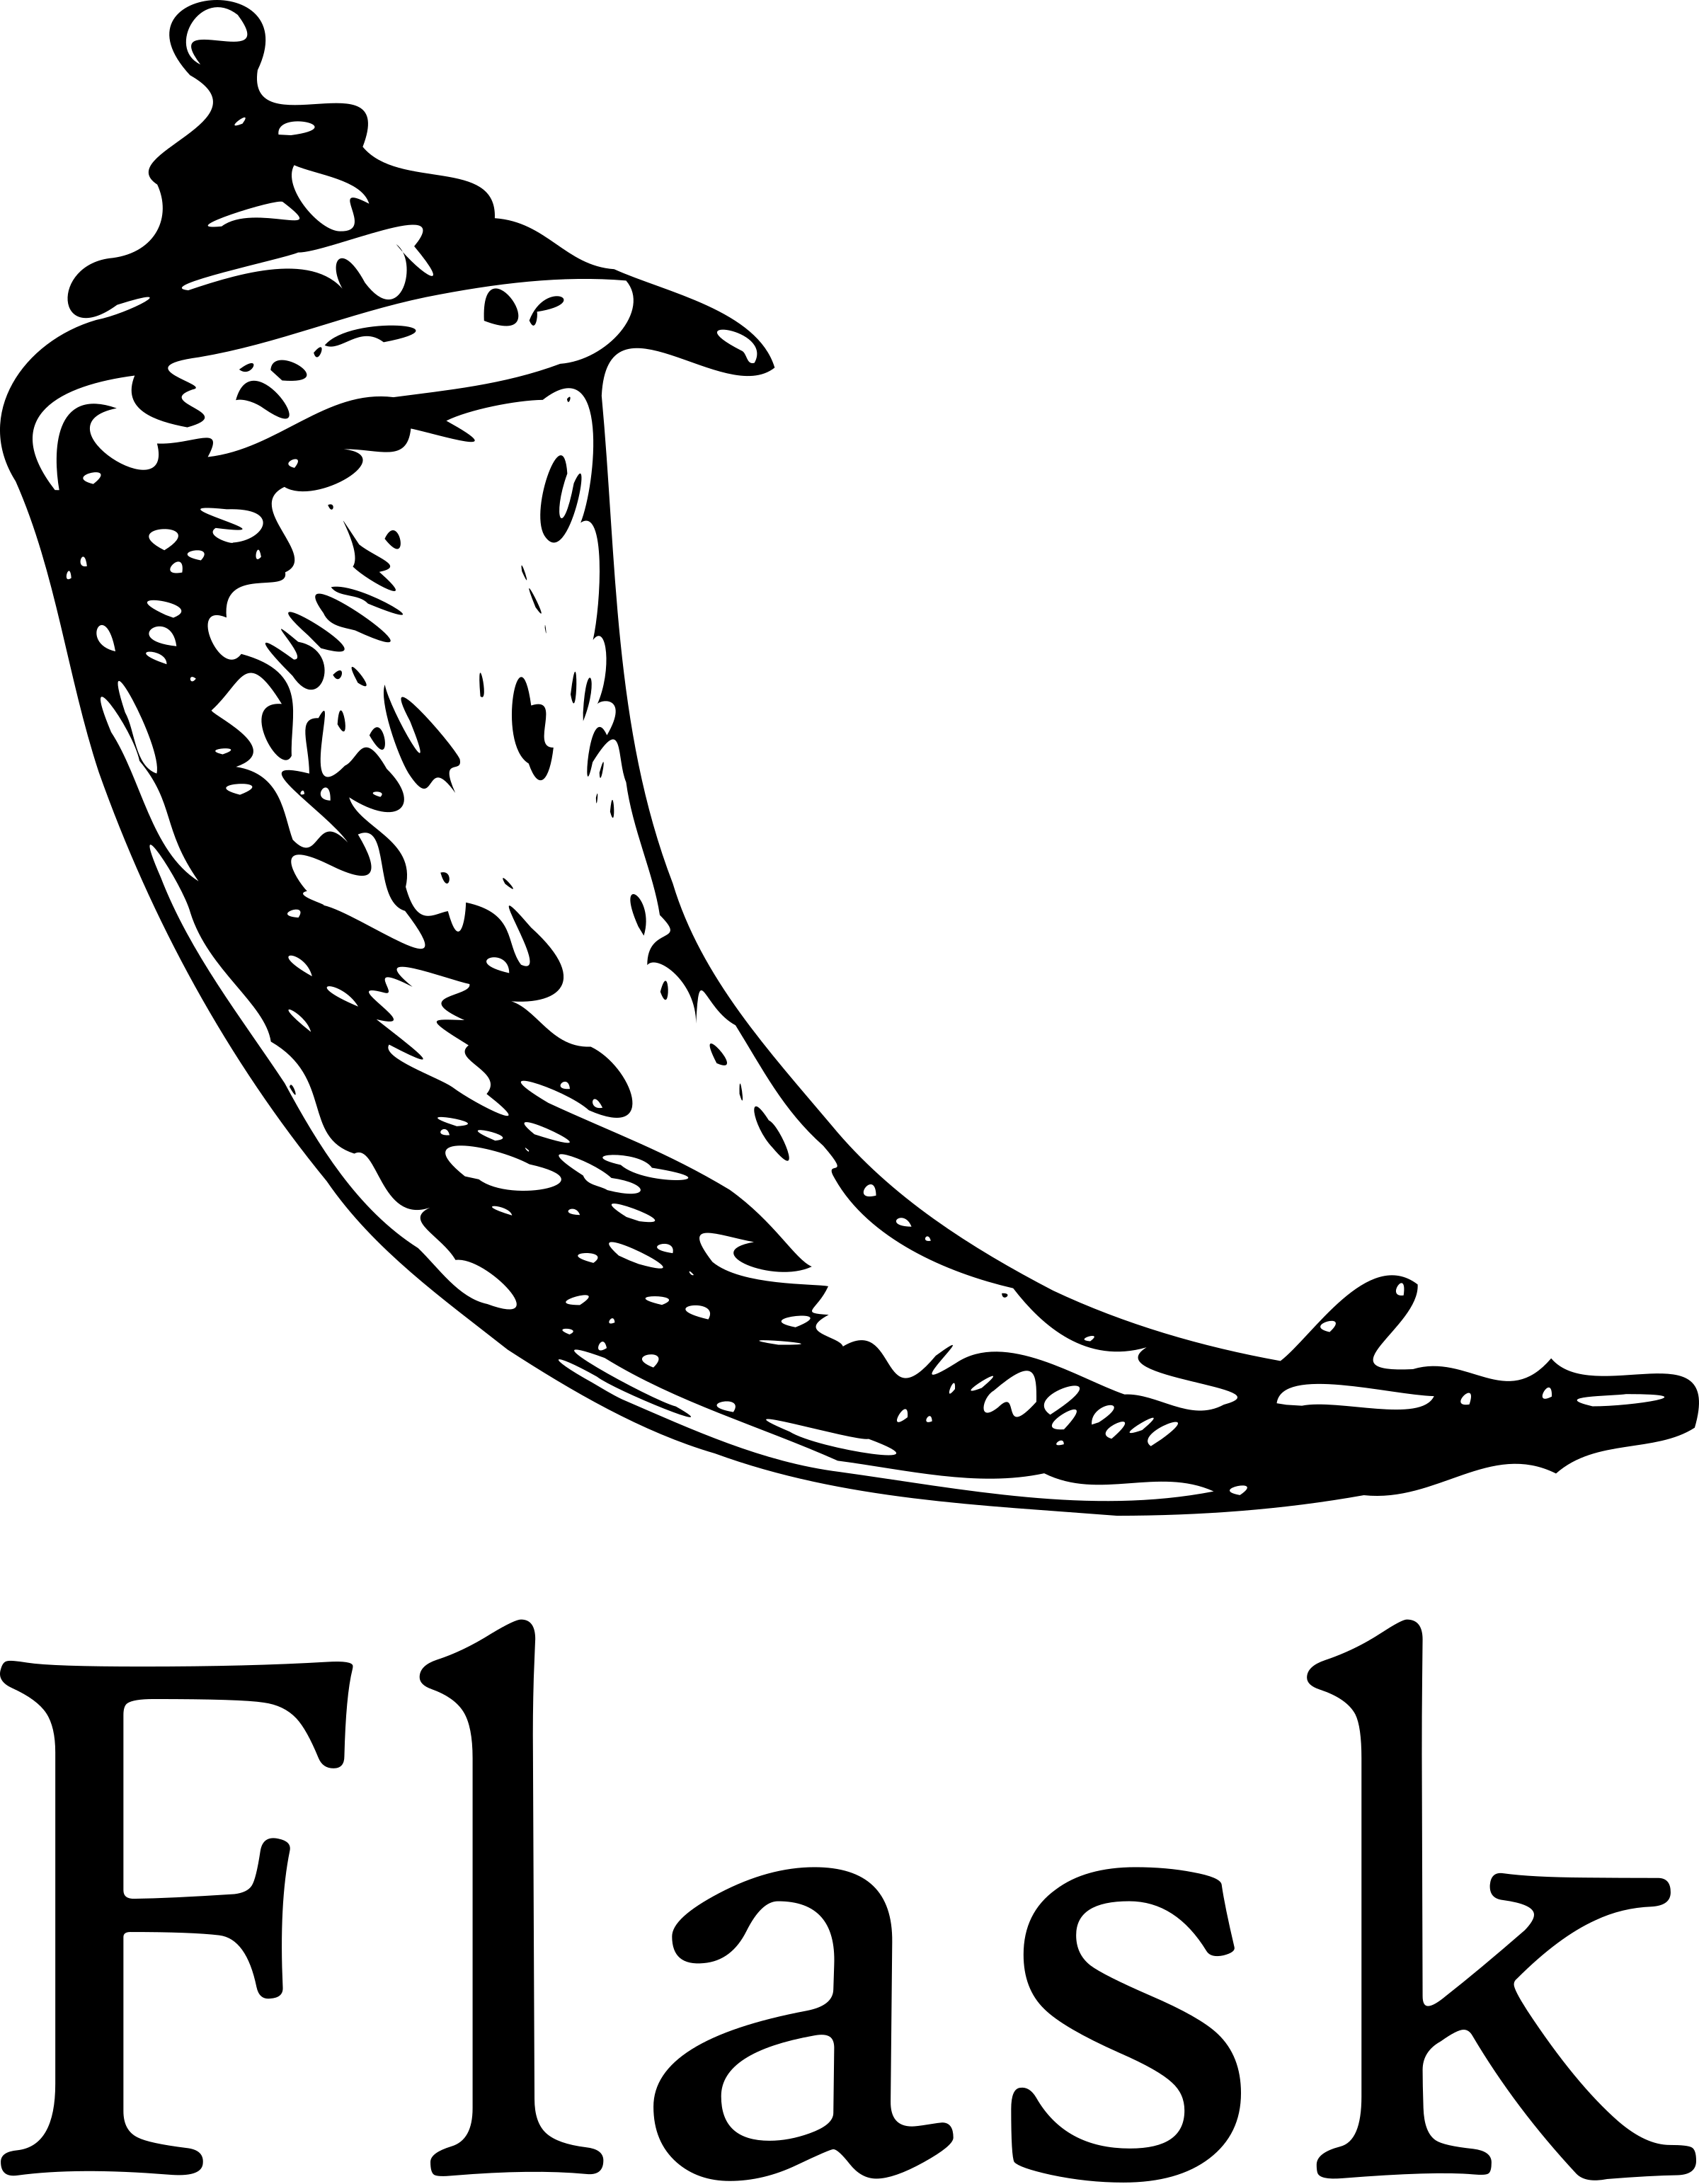
\includegraphics[width=40.38pt,height=52.5pt]{img/flask.png}};
        %Straight Lines [id:da3933293266418665]
        \draw    (239.98,93) -- (239.52,159) ;
        \draw [shift={(239.5,162)}, rotate = 270.4] [fill={rgb, 255:red, 0; green, 0; blue, 0 }  ][line width=0.08]  [draw opacity=0] (8.93,-4.29) -- (0,0) -- (8.93,4.29) -- cycle ;
        \draw [shift={(240,90)}, rotate = 90.4] [fill={rgb, 255:red, 0; green, 0; blue, 0 }  ][line width=0.08]  [draw opacity=0] (8.93,-4.29) -- (0,0) -- (8.93,4.29) -- cycle ;
        %Straight Lines [id:da24057878811893751]
        \draw    (167.75,200.25) -- (203.75,200.25) ;
        \draw [shift={(206.75,200.25)}, rotate = 180] [fill={rgb, 255:red, 0; green, 0; blue, 0 }  ][line width=0.08]  [draw opacity=0] (8.93,-4.29) -- (0,0) -- (8.93,4.29) -- cycle ;
        \draw [shift={(164.75,200.25)}, rotate = 0] [fill={rgb, 255:red, 0; green, 0; blue, 0 }  ][line width=0.08]  [draw opacity=0] (8.93,-4.29) -- (0,0) -- (8.93,4.29) -- cycle ;
        %Straight Lines [id:da10061083103025648]
        \draw    (283.75,199.58) -- (318.5,199.58) ;
        \draw [shift={(321.5,199.58)}, rotate = 180] [fill={rgb, 255:red, 0; green, 0; blue, 0 }  ][line width=0.08]  [draw opacity=0] (8.93,-4.29) -- (0,0) -- (8.93,4.29) -- cycle ;
        \draw [shift={(280.75,199.58)}, rotate = 0] [fill={rgb, 255:red, 0; green, 0; blue, 0 }  ][line width=0.08]  [draw opacity=0] (8.93,-4.29) -- (0,0) -- (8.93,4.29) -- cycle ;
        %Image [id:dp8556439958741602]
        \draw (567,186) node  {
\includegraphics[width=52.5pt,height=52.5pt]{img/user.png}};
        %Straight Lines [id:da26821981951432505]
        \draw    (385.5,184.58) -- (499.5,184.58) ;
        \draw [shift={(502.5,184.58)}, rotate = 180] [fill={rgb, 255:red, 0; green, 0; blue, 0 }  ][line width=0.08]  [draw opacity=0] (8.93,-4.29) -- (0,0) -- (8.93,4.29) -- cycle ;

        %Straight Lines [id:da7643998387312995]
        \draw    (388.5,214.58) -- (412.5,214.58) -- (500.5,214.58) ;

        \draw [shift={(385.5,214.58)}, rotate = 0] [fill={rgb, 255:red, 0; green, 0; blue, 0 }  ][line width=0.08]  [draw opacity=0] (8.93,-4.29) -- (0,0) -- (8.93,4.29) -- cycle ;
        %Straight Lines [id:da5051570254396728]
        \draw    (240.5,256) -- (240.5,278) ;
        \draw [shift={(240.5,281)}, rotate = 270] [fill={rgb, 255:red, 0; green, 0; blue, 0 }  ][line width=0.08]  [draw opacity=0] (8.93,-4.29) -- (0,0) -- (8.93,4.29) -- cycle ;
        \draw [shift={(240.5,253)}, rotate = 90] [fill={rgb, 255:red, 0; green, 0; blue, 0 }  ][line width=0.08]  [draw opacity=0] (8.93,-4.29) -- (0,0) -- (8.93,4.29) -- cycle ;
        %Rounded Rect [id:dp9694318857670313]
        \draw   (2,25.5) .. controls (2,15.28) and (10.28,7) .. (20.5,7) -- (464,7) .. controls (474.22,7) and (482.5,15.28) .. (482.5,25.5) -- (482.5,300.5) .. controls (482.5,310.72) and (474.22,319) .. (464,319) -- (20.5,319) .. controls (10.28,319) and (2,310.72) .. (2,300.5) -- cycle ;
        %Image [id:dp9562999520117128]
        \draw (99,377) node  {
\includegraphics[width=52.5pt,height=52.5pt]{img/tablet.png}};
        %Straight Lines [id:da22030012036466173]
        \draw    (98.5,295) -- (186.5,295) ;
        \draw [shift={(189.5,295)}, rotate = 180] [fill={rgb, 255:red, 0; green, 0; blue, 0 }  ][line width=0.08]  [draw opacity=0] (8.93,-4.29) -- (0,0) -- (8.93,4.29) -- cycle ;

        %Straight Lines [id:da28839463654139263]
        \draw    (98.5,295) -- (98.5,339) ;
        \draw [shift={(98.5,342)}, rotate = 270] [fill={rgb, 255:red, 0; green, 0; blue, 0 }  ][line width=0.08]  [draw opacity=0] (8.93,-4.29) -- (0,0) -- (8.93,4.29) -- cycle ;

        %Straight Lines [id:da2120925552884272]
        \draw  [dash pattern={on 0.84pt off 2.51pt}]  (154.75,380.58) -- (473.5,380.58) ;

        \draw [shift={(151.75,380.58)}, rotate = 0] [fill={rgb, 255:red, 0; green, 0; blue, 0 }  ][line width=0.08]  [draw opacity=0] (8.93,-4.29) -- (0,0) -- (8.93,4.29) -- cycle ;
        %Image [id:dp7151280650926004]
        \draw (535.32,366) node  {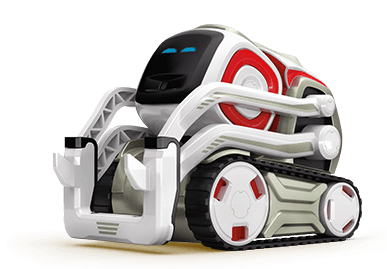
\includegraphics[width=96.27pt,height=69.12pt]{img/cozmo.png}};
        %Straight Lines [id:da948112813701837]
        \draw  [dash pattern={on 0.84pt off 2.51pt}]  (151.75,402.58) -- (470.5,402.58) ;
        \draw [shift={(473.5,402.58)}, rotate = 180] [fill={rgb, 255:red, 0; green, 0; blue, 0 }  ][line width=0.08]  [draw opacity=0] (8.93,-4.29) -- (0,0) -- (8.93,4.29) -- cycle ;

        %Image [id:dp8991970614844648]
        \draw (332,113) node  {
\includegraphics[width=36pt,height=36pt]{img/tensorflow.png}};
        %Straight Lines [id:da8686562029937168]
        \draw    (257.5,118) -- (297.5,118) ;
        \draw [shift={(300.5,118)}, rotate = 180] [fill={rgb, 255:red, 0; green, 0; blue, 0 }  ][line width=0.08]  [draw opacity=0] (8.93,-4.29) -- (0,0) -- (8.93,4.29) -- cycle ;

        %Straight Lines [id:da7903500333471788]
        \draw    (257.5,118) -- (257.5,165) ;


        %Straight Lines [id:da017309376357115047]
        \draw    (557.15,117.91) -- (557.15,93) ;
        \draw [shift={(557.15,90)}, rotate = 450] [fill={rgb, 255:red, 0; green, 0; blue, 0 }  ][line width=0.08]  [draw opacity=0] (8.93,-4.29) -- (0,0) -- (8.93,4.29) -- cycle ;

        %Straight Lines [id:da46777924457369235]
        \draw    (557.15,117.91) -- (453.67,117.91) ;


        %Image [id:dp9871015067821471]
        \draw (559,44) node  {
\includegraphics[width=42pt,height=42pt]{img/analysis.png}};

        % Text Node
        \draw (569,227) node  [font=\footnotesize] [align=left] {Human-Robot Interaction};
        % Text Node
        \draw (435,175) node  [font=\footnotesize] [align=left] {Image};
        % Text Node
        \draw (436,204) node  [font=\footnotesize] [align=left] {Commands};
        % Text Node
        \draw (114,22) node   [align=left] {\textbf{Development Machine}};
        % Text Node
        \draw    (196.5,282.5) -- (287.5,282.5) -- (287.5,307.5) -- (196.5,307.5) -- cycle ;
        \draw (242,295) node   [align=left] {Cozmo SDK};
        % Text Node
        \draw (100,423) node   [align=left] {\textbf{Android Device}};
        % Text Node
        \draw (120,276) node   [align=left] {{\footnotesize ADB}};
        % Text Node
        \draw (323,420) node   [align=left] {Wi-Fi Connection};
        % Text Node
        \draw (536,420) node   [align=left] {\textbf{Cozmo}};
        % Text Node
        \draw (319,370) node  [font=\footnotesize] [align=left] {Image};
        % Text Node
        \draw (320,394) node  [font=\footnotesize] [align=left] {Commands};
        % Text Node
        \draw (396,119) node   [align=left] {TensorBoard};
        % Text Node
        \draw (559,75) node  [font=\footnotesize,] [align=left] {Data Analysis};
        % Text Node
        \draw (241,242) node   [align=left] {OpenAI Gym};


    \end{tikzpicture}
    }
    \caption[Interaction Human/Robot]{Interaction between the user and Anki Cozmo.
        The main Python script utilises OpenAI Gym for the reinforcement learning component and PyTorch for the deep learning one.
        The user can influence with the flow of the system through a simple web app that interacts directly with OpenAI Gym and the Cozmo SDK to provide information for the user (e.g.\ images, learning information) and the robot (e.g.\ commands).
        The last component consists in TensorBoard thanks to the script can store results that can be retrieved later by the user.}
    \label{fig:system}
\end{figure}

\subsection{Human-Robot Interaction} \label{subsec:human-robot-interaction}

It is noticeable that the simulator can undoubtedly be programmed to understand whenever the car is going outside the track, crossing the roadside.
In a reinforcement learning scenario, this fact facilitates the restarting procedure for an episode: the developer has to bind some events or actions to a process that stops the current episode, put the car on the road again and starts the next experiment.
In the real world, the situation is more complicated not only because of the need of the human intervention to relocate the car in a safe place but also because there are more variables to take into account.
The most critical factor is that the failure of an episode in the simulator has no threats or costs, while real-world experiments failures could lead to high costs and severe damage to the car and equipment.
Despite this point, the application of such experiment typology in a real environment instead of a mere simulation represents an exciting challenge that could bring reinforcement learning to the next level.
In order to make experiments as safe as possible, the authors of~\cite{kendall2018learning,kendall2019learning} implemented a self-driving system designed explicitly for self-driving reinforcement learning experiments where the car driver has the faculty of stopping the car when it is going to run off the road or in a dangerous situation and relocating it in the nearest safe position to start the next learning episode.
By simply pressing a button, the logic of the car disables reinforcement learning algorithm decision and gives full control to the real driver of the car.

We aimed to implement this kind of user-robot interaction also in our setup.
The requirements were almost the same as the ones described in the paper, but this case could not rely on steering wheel, brakes and accelerator as in the car scenario where they are directly accessible by the user.
The system needed an interface to allow the user to stop the robot whenever it is approaching the side of the road and manoeuvre the robot just like a car.

For this reason, we firstly implemented a straightforward interface using a web app implemented using plain HTML5, CSS3 and Javascript for the frontend and Flask \footnote{Flask Github Repository: \href{https://github.com/pallets/flask}{https://github.com/pallets/flask}}, a lightweight Web Server Gateway Interface (WSGI) web application framework, as backend.
Therefore, we designed the web-app interface by using the Bootstrap framework \footnote{Bootstrap documentation: \href{https://getbootstrap.com/}{https://getbootstrap.com/}} to offer an easy-understandable and appealing user experience.

The aim of this application is allowing user interaction with Cozmo and Flask represented the right choice to allow the communication between this interface and the OpenAI Gym environment.
The Flask backend interacts directly with the functions offered by Cozmo SDK to allow the user to see the live streaming from Cozmo camera directly in the web app.
Therefore it can receive, convert and forward commands from the robot to the SDK.
These commands consist of the pressure of both single or combination of buttons: Flask decides the action to trigger programmatically with hard-coded conditions and calculates speeds and accelerations of both right and left treads.

The SDK function we utilised to control Cozmo is \texttt{drive\_wheels()}.
The parameters of this function are the following:

\begin{itemize}
    \item \textbf{\texttt{l\_wheel\_speed}} (\textit{float}): mandatory parameter that specifies the speed of the left tread (in millimeters per second).
    \item \textbf{\texttt{r\_wheel\_speed}} (\textit{float}): mandatory parameter that specifies the speed of the right tread (in millimeters per second).
    \item \textbf{\texttt{l\_wheel\_acc}} (\textit{float}): optional parameter that specifies the acceleration of the left tread (in millimeters per second squared).
          The default value is the equal to \texttt{l\_wheel\_speed}.
    \item \textbf{\texttt{r\_wheel\_acc}} (\textit{float}): optional parameter that specifies the acceleration of the right tread (in millimeters per second squared).
          The default value is the equal to \texttt{r\_wheel\_speed}.
    \item \textbf{\texttt{duration}} (\textit{float}): it specifies the duration of the driving action of the robot.
          It calls \texttt{stop\_all\_motors()} after this duration has passed.
          The default value is \texttt{None}, in this case, the behaviour of this function is equivalent to the non-async \texttt{drive\_wheel\_motors()} one: the wheels will continue to move at that speed until commanded to drive at a new speed.
\end{itemize}

This method is the same we used to implement the OpenAI Gym environment, allowing the algorithm to interact with the robot just like a human in the driving seat.
Just as examples, the user can start and stop the episode using the enter button, forget the previous episode with backspace and relocate the robot on the track using W, A, S and D buttons.

In this context, the human-robot interaction has a crucial role in the learning process.
It represents the source of all improvements and imperfections of learning process results: the robot learns which actions are valuable and which are unprofitable or disadvantageous, but it is essential to remember that the human is the one who decides the correctness of each action by stopping the car in a dangerous situation.
This fact leads to the introduction of unconscious bias in the algorithm that could affect final results.
We will discuss the experiments and their results thoroughly in \vref{ch5,ch6}.

\subsection{OpenAI Gym Cozmo Environment}

This section describes the main features we implemented in \textit{CozmoEnv}, the OpenAI Gym environment we developed to apply and test reinforcement learning algorithms with Cozmo.

\subsubsection{MDP formalisation}

The first important step to implement a reinforcement learning environment is formalising the problem we want to solve as a Markov Decision Process (MDP).
Starting from the definition of MDP that we already reported in~\vref{eq:mdp}, we studied and investigated the best configuration to provide an acceptable trade-off between performance and memory consumption, capable of making the system work on the development machine we used for our experiments.
In the following paragraphs, we will analyse each MDP aspects paying particular attention to the problems we faced and the motivations behind every decision made to overcome them.

\paragraph{State/Observation Space} The environment observation is the group of information that the reinforcement learning agent can see and obtain from the interaction with the real world.
In the self-driving tasks in question, the most reasonable way to obtain knowledge about the surrounding environment is to exploit front camera images provided by Cozmo SDK.
However, it is essential to remember that the state must satisfy the Markov property according to which it must be independent of the past given the present.
Using a single image to describe the current state may be an oversimplification of the problem.
Even a human would not be able to determine the best action to take starting from a single frame.
That is because it is difficult to infer or determine the current direction of the car, speed or steering wheel position.
Merely adding another image can intuitively improve the human perception of the scene: as an example, the first intuition this introduction could reveal is where the car is going.

To verify this fact before starting the experiments with the application of the reinforcement learning algorithms to Cozmo, we firstly analysed the results of some experiments on the environment of the classic control problem of trying to keep a frictionless pendulum standing up (\textit{Pendulum-v0}).
The original version of this environment utilises angle position and trigonometric results as observation to return to the agent.
In order to make this environment suitable for convolutional neural networks, we decided to appropriately modify it to exploit raw images as observations instead of the original information.
We noticed that the usage of a single image as observation leads to unstable and worse results than the ones obtained by combining two subsequential images to feed the algorithm.
For this reason, we decided to use two consecutive raw images provided by Cozmo by using a queue data structure with size two.
In the code flow, the developer merely has to push the next image obtained by the robot and use the specific queue function implemented to obtain the concatenation of the last two images, only when necessary.

Therefore, we decided to reduce the original size of the input Cozmo image to 64$\times$64.
We made this decision as a trade-off between performance, learning phase duration and space available in the central memory to store the replay memory.

In conclusion, the observation provided to the agent is the concatenation of two images with dimension 64$\times$64 pixels.

\paragraph{Action Space}

Another essential part that we needed to formalise is the action space, how the agent can interact and influence the surrounding environment.
In the car scenario, the two main components of driving are the speed of the vehicle and the position of the steering wheel.
To straightforwardly formalise these two parts, we decided to use two simple real values.

We chose to define the desired speed value in a range of 0 to 1, while we opted for a range of -1 to 1 for the steering wheel position.
These limits allow the agent to manipulate simple values in the decision-making process and to facilitate the manipulation of neural network results.
At the same time, the underlying logic of the environment takes care to translate these values into a compatible format for the Cozmo SDK.
Indeed, as we reported previously in this section, the Cozmo SDK function exploited to manoeuvre the robot needs at least the speed of each tread.
\Vref{conversionCozmoEnv} reports key steps of this translation.
Therefore we decided to raise acceleration parameters by setting them equal to 4 times the desired speed of each thread.

\begin{algorithm}[!h]
    \SetAlgoLined
    \small
    \DontPrintSemicolon
    \LinesNumbered
    \KwIn{Desired speed $s_t \in \{ x \in \mathbb{R} | 0 \le x \le 1 \}$\newline Steering wheel position $w_t \in \{ x \in \mathbb{R} | -1 \le x \le 1\} $\newline Maximum forward speed $s^{\text{forward}}_{\text{max}} = 150\text{mm/s}$\newline Maximum turning speed $s^{\text{turning}}_{\text{max}} = 100\text{mm/s}$}

    Left tread speed: $ts_{\text{left}} = s_t \cdot s^{\text{forward}}_{\text{max}} + w_t \cdot s^{\text{turning}}_{\text{max}}$\;
    Right tread speed: $ts_{\text{right}} = s_t \cdot s^{\text{forward}}_{\text{max}} - w_t \cdot s^{\text{turning}}_{\text{max}}$

    \KwOut{Left tread speed $ts_{\text{left}}$ \newline Right tread speed: $ts_{\text{right}}$}
    \caption{CozmoEnv actions conversion from virtual to real}
    \label{conversionCozmoEnv}
\end{algorithm}


\paragraph{Reward Function}

The reward function is the crucial feature to define in the formalisation of the MDP.
After a review of the available literature and the analysis of the problem, we obtained a list of ideas and concepts to model the reward function:

\begin{itemize}
    \item \textbf{Lane Distance}: this model calculates the reward of each action by calculating the distance between the car and the centre of the lane.
          The main aim is to prioritise the correct positioning of the car on the lane, crucial for driving safety.
          However, it is noticeable that this value can be easily calculated in a simulated environment, while it needs a lot of sensors and calculation to obtain a good estimation in a real-world environment.
          Beyond this problem, this approach has difficulties in scaling to varying environments where road typology and dimension is not a pre-configured constant.
          Therefore, it is a limited approach because, clearly, human beings do not always drive the car in the perfect centre of the lane: for instance, when approaching a curve it could be more convenient to move the car from slightly away from the perfect centre.

          This fact reveals the shortcomings of this approach: the system can perform only as good as the human intuition underlying the hand-crafted lane reward.

    \item \textbf{Distance Covered}: the second approach we investigated was the one suggested by~\cite{kendall2018learning,kendall2019learning}, where the reward of a specific action consists of the total distance covered by the car for each specific action taken.
          Approaching the problems with this method leads to results that can be easily understandable for humans: indeed, the total reward of each episode represents the total distance travelled by the robot.

          In the car scenario of the previously mentioned publication, it is possible to use the car odometry device to quickly retrieve this value after each action and calculate the reward of a specific decision obtaining the difference with the previous value.
          Cozmo does not have such kind of sensor on board.
          Therefore it is necessary to calculate this value manually.
          The intuition behind a reasonable estimation of the distance covered by Cozmo consists of using the fundamental formula of kinematics: the speed.
          Indeed, in the designed system, we have direct access to the aspired speed because it is a parameter that the agents decide at each iteration, and it is possible to derive the time elapsed between one action and its following one by manually calculating them inside the OpenAI Gym environment.

    \item \textbf{Speed Crash Penalty}: the third typology of reward we investigated consists of a sort of life bonus reward.
          The robot receives a reward (e.g./ 1 point) for each timestep of correct decisions and a negative reward (e.g./ -10 points) every time the user stops the robot preventing the crash.
          Therefore we added to the positive reward a small quantity that depends on the current speed to encourage the robot to stay on track and increase its speed.
          Consequently, we decided to add a penalty in faulty time step proportional to the robot crash speed to entice the robot in avoiding high speed when close to critical points.
          \Vref{eq:speedCrashPenalty} formalises the reward used in this environment: $p_1$ and $p_2$ are two parameters that determine how much the speed influence the reward and their module must be much less than the constant value in the equation to highlight the fact that they represent a secondary objective \cite{raffin2019learning}.
          \begin{equation}
              r_t = \begin{cases}
                  +1 + p_1 \cdot s_t, & \mbox{if } \mbox{Cozmo on the track} \\ -10 - p_2 \cdot s_t, & \mbox{if } \mbox{Cozmo off the track}
              \end{cases}
              \label{eq:speedCrashPenalty}
          \end{equation}

\end{itemize}

After the analysis of these three reward design proposal, we decided to select the second one to pursue our experiments in the real world.
As previously reported, the first option would have been hard to carry on and to scale up.
The third option hints intriguing facts that a reinforcement learning agent could take into account to better solve the driving task of our experiments.
The only withdrawal of this approach is related to the correlation between reward and distance covered: this correspondence is significant for the developer to have a more transparent overview of what is happening and how the algorithm is learning.
In the second option, the distance covered by the robot is equal to the reward, while this conformity is lacking in the third option.
For this reason, we decided to take the second reward proposal for this time.
We noticed that it could be an exciting future development trying to merge the second alternative with the third one to obtain a brand new reward function that both penalises bad decisions proportionally to speed and maintain its correspondence with the track crossed.

In the first implementation of the environment, the agent was able to make decisions without a specific timing between actions.
This fact led to different problems in the implementation of reinforcement learning agents.
The first problem was related to experience memory gathering also caused by the limitation of Cozmo Camera: it is a 30fps camera but, as reported in the documentation of Cozmo SDK, the Cozmo framework emits a new camera image generally up to 15 times per second.
Therefore, the frequency of image requests was very high because the system did not contain timing implementation constraints in the control of operations.
These two factors led the system to retrieve the same image both before and after taking the current action.

Consequently, the state of each environment step consisted of the concatenation of two images that were often the same picture.
This consequence led to a conceptual error that may influence the process of learning if we observe that with a human perspective: a state of this kind represents an action that does not influence the environment of the system whilst it is modifying it.
We noticed this problem because, in the first part of the experiments, where the agent takes random action to explore the surrounding environment, the robot continued to drive a straight path, even if shaky, without taking a definite step in a specific direction and with an almost constant speed.
This symptom was strictly related to the robot's inability to have the right time to carry out a specific action before interacting with the environment with the next action.
Accordingly, the robot ends up navigating with an average speed close to the half of the maximum speed and always going in a straight line only with small and temporary slopes to the right or left.
After noting this problem, we fixed it by hard-coding a minimum interval between the execution of a specific action and the beginning of the next one in the OpenAI Gym environment: we selected this value according to the constraint given by the Cozmo SDK about robot camera device.

\subsubsection{Neural networks and hyperparameters}

Another essential component in the developing of the control system is the convolutional neural network we designed.
As already reported in chapter 3, we opted using PyTorch as deep learning framework.
To choose the neural network that could better meet the requirements, we analysed the models used in~\cite{lillicrap2015continuous,kendall2018learning,haarnoja2018soft, haarnoja2018alg}.

The author in~\cite{lillicrap2015continuous} presented two types of neural networks, but the model we are interested in is the convolutional one, used to learn from pixels.
It consists of 3 convolutional layers without pooling with 32 filters at each layer.
Therefore, the authors added two fully connected layers with 200 units.
The paper also contains information about the initialisation of network weights and biases: they set final layer ones from a uniform distribution of $[-3\times 10^{-3},3\times 10^{-3}]$ and $[-3\times 10^{-4},3\times 10^{-4}]$ respectively in order to ensure the initial outputs for the policy and value estimates were near zero.
They used uniform distributions $[\frac{-1}{f^{0.5}}, \frac{1}{f^{0.5}}]$ where $f$ is the layer fan-in.
The actions were concatenated just before fully connected layers.

In \cite{kendall2018learning}, the authors used a small convolutional neural network with four convolutional layers, with 3$\times$3 kernels, a stride of 2 and 16 feature dimensions, shared between the actor and critic models.
Therefore, the flattened encoded state obtained from convolutional operations were used as input for fully connected layers of both actor and critic: in the last case, it was concatenated with the actions.
In this architecture, there was only a single fully-connected layer of 8 features.
They conducted the experiments using a modified Renault Twizy vehicle with a single forward-facing video camera situated in the centre of the roof at the front of the car, carrying out their experiments on-board using a single NVIDIA Drive PX2.
They managed to solve their self-driving task in a handful of trials using 250 optimisation steps with a batch size of 64.
They managed to make the experiment very manageable with an optimisation phase that took approximatively 25 seconds, which is a reasonable amount of time considering that the driver must reposition the car at the centre of the lane before restarting the procedure.
As stated in the paper, their agent was able to cover a distance of about 300 metres in 37 minutes of training time within just 35 episodes.
In the real world, the environment is much more complicated than the simulated one, and then they decided to implement the logic of the agent through the usage of a Variational Autoencoder (VAE).
This decision led to an improvement in the reliability of the algorithm.

In \cite{haarnoja2018alg}, the authors reported the training of a real-world robotic task with a 3-finger dexterous robotic hand.
The objective of the agent is to position a sink faucet in a specific position highlighted by a coloured end.
The neural network exploited on this occasion consisted of two convolutional layers with 3$\times$3 filters and max-pool layers, four features and followed by two fully connected layers with 256 units.
Even in this case, the authors exploited RGB images to carry out real-world training of the agent.
Therefore, they included some information about training time: the agent needed 300k environment interaction steps with an equivalent of 20 hours of training.

The problems just outlined have relative differences, but the varying durations of the experiments are truly impressive.
This fact underlines how the training duration depends not only on the data quality but also on hyper-parameters used, on the complexity of the problem and the available computational power.
It is the primary motivation behind the complexity of an experiment carried out entirely in the real-world.

After the analysis of the neural network used in the last-mentioned papers, we tried to modify these models after trying them on the modified Pendulum environment provided by the OpenAI Gym framework and analysing training and testing results.
We exploited the network architectures that passed this selection to made experiments with \textit{Pendulum-v0} and, consequently, with the environment we designed with Cozmo.

However, before finding a good architecture to exploit, we started little experiments with Cozmo to analyse changes in the behaviour policy of the robot.
There we noticed a crucial factor to take into account to decide what network to use for our experiment: the optimisation phase duration.
It is a vital parameter to make the experiment manageable for the user: in this thesis work, the agent is not in a simulation where the computer automatically decides when to restart the episode so that the human can let the experiment running by itself.
In this context, the user must be ready to stop, reposition and restart the car in a specific moment.
Given the evidence that an experiment like this could last thousands of episodes, we aimed to reduce the waiting time for the user to make the experiments last less, or, at least, obtain a good relationship between the duration of the episode and that of the optimisation steps.
To avoid a long waiting time after each episode, we tried to spread the optimisation phase inserting a single learning step after each action taken by the agent. We found out this approach in some implementation of DDPG algorithm mainly applied to simulated environments. This choice seemed working with the \textit{Pendulum-v0} task because, in a simulated context, the environment stops itself waiting for the next action taken by the agent during the optimisation phase: the system flow is independent of the duration of the last-mentioned phase.
It is noticeable that this fact does not apply to a real-world scenario like the one we implemented with Cozmo. As we discussed before in this chapter, the robot continues the drive also during the learning process.
Therefore the system is highly unstable because this process not always has the same length and every action lasts differently: it depends on the specific network topology.
After the analysis of this behaviour, we decided to maintain the optimisation phase among episodes and to fix a specific duration for each action of Cozmo.

The architecture we selected was a sort of merge of the ones we found in \cite{kendall2018learning,kendall2019learning,haarnoja2018alg}. We opted for a neural network with 3 convolutional layer with 16 features. We decided to use a stride of 2 instead of using pooling layers \cite{springenberg2014striving}. The last part of the architecture is composed by two fully-connected layer with an hidden size of 256 features.



\subsubsection{Data Analysis}

\subsection{Reinforcement learning algorithms implementations}



% \todomacaluso{
% 	\begin{itemize}
% 		\item Introduction to the chapter
% 		\item General description of the control systems with a diagram representing all the technologies involved.
% 		\item Setup of the algorithms (DDPG, SAC)
% 		      \begin{itemize}
% 			      \item We decided to rewrite both algorithms without using libraries directly.
% The first motivation was didactical, implementing from scratch is helpful to understand the practical implementation of the algorithm better, but also to make it possible to implement the singularity of the real Cozmo environment.
% 			      \item The interaction with OpenAI Gym and PyTorch
% 			      \item Discussion about Hyper-Parameters and the problems faced in the real world situation in the selection of these parameters.
% 		      \end{itemize}
% 		\item Setup and implementation of CozmoEnv
% 		      \begin{itemize}
% 			      \item Technologies used to implement the interaction between the Cozmo SDK and OpenAI Gym.
% 			      \item Differences from the simulated environment caused by the need for direct human interaction.
% 			      \item Implementation of human interaction in the system.
% 		      \end{itemize}
% 		\item Setup of the real Environment
% 		      \begin{itemize}
% 			      \item The Track design
% 			      \item Analysis of the problems:
% 			            \begin{itemize}
% 				            \item Reflection
% 				            \item Background and Horizon
% 			            \end{itemize}
% 			      \item (Single Line Track)
% 		      \end{itemize}
% 	\end{itemize}
% }

% \section{The track}

% The design and training of a good driving model cannot go beyond the construction and design of the road.
%For this reason, some time was spent searching the better way to build a path where to train Cozmo.
% This section aims to present the central concept and decisions made about the design of the track for the experiments, starting from the materials used, up to the description of the dimensional choices applied.

% \subsection{Track requirements}

% It is essential to explain the primary needs of the road before proceeding with the description of the choices made.

% Firstly, the track needs to be easily transportable to allow various attempt with different locations and environmental conditions that could affect the training phase.
%In particular, it is necessary to use a material less reflective as possible to avoid problems during the learning process.
% Another crucial factor is the dimension of the lane, which must reproduce an environment similar to the real one.
% It can be done analyzing the ratio of the size of a vehicle to the width of a road.
% On average, a family car is about $160$-$170$cm large, while a lane width can vary between $275$cm and $375$cm.
% Cozmo width is about $5.5$cm, which results in a ratio of $1/30$.
% Therefore, the scaled lane must be between $9$cm and $12.5$cm.

% \subsection{Track design and materials}

% The first choice to make is the one about the type of material to use as terrain for the track.
% The first choice was the black floor of the Data Science laboratory of Eurecom.
% It was useful only during the initial design and development of the control system to build small pieces of track in which testing functionalities.
% This solution had numerous drawbacks such as the impracticality to transport and high light reflection.


% The following list provides a brief report of the various solutions taken into account during the thesis, together with an analysis of advantages and drawbacks.

% \begin{itemize}
% 	\item \textit{Covering fabric}: this material is easily transportable, but it has a high light reflection, and its structure is prone to make wrinkles and dunes challenging to remove.
% 	\item \textit{Tar paper}: this solution slightly diminished the reflection problem compared to the previous choice, but the material was fragile and with the same drawbacks of the covering fabric.
% 	\item \textit{Cotton fabric}: this solution offers an easily  transportable material with reduced light reflection where it is easy to remove wrinkles and dunes.
% \end{itemize}

% Summing up, it is noticeable from this analysis that the cotton fabric provides the right trade-off among all requirements reported before.

% The structure of the road is also composed by the lane.
% The implementation of this part was done using a simple paper tape of width equal to $2.5$cm. As described in the beginning of this section, the width of the lane must be between $9$cm and $12.5$cm to provide a context similar to the real one. Because of the narrow and limited angle of vision provided by Cozmo camera, $10$cm-width was set: positioning the tape with a distance greater than $10$cm would result in a great part of the tape outside the view of the camera.